\section{Experiments and Results}
\label{sec:experiments}

\subsection{Headline results}
\label{sec:headline}

Table~\ref{tab:headline} and Figure~\ref{fig:forest} summarize the run's
findings. Under the pre-registered protocol the verdict machinery returned
the category \emph{hurts} on both architectures; the binding F12 downgrade
rule (Section~\ref{sec:method-verdict}) converts the reportable claim to
\textbf{no evidence of benefit under the affordable tuning budget}, with the
raw numbers reported alongside. The load-bearing mechanism control is null
on both architectures: MP-eigenselection is statistically indistinguishable
from a norm- and $k$-matched random-subspace projection (equivalence at
$\pm 0.004$ resolution). The independent audit re-execution (fresh seeds,
independently constructed evaluation shard) reproduces both findings.

\begin{table}[t]
\centering
\footnotesize
\setlength{\tabcolsep}{2.5pt}
\begin{tabular}{llcl}
\toprule
Comparison & Estimate & 95\% CI (MBB, $L{=}4$) & Reading \\
\midrule
\multicolumn{4}{l}{\emph{Headline: filter-on $-$ filter-off (vs.\ tuned AdamW)}} \\
\quad MLP, seeds 0--2 (exp-004) & $-0.00527$ & $[-0.00886, -0.00181]$ & hurts $\to$ F12 downgrade \\
\quad GRU, seeds 0--2 (exp-005) & $-0.00484$ & $[-0.00758, -0.00211]$ & hurts $\to$ F12 downgrade \\
\quad MLP re-run, seeds 10--12, producer shard & $-0.00546$ & $[-0.00892, -0.00204]$ & reproduces \\
\quad MLP re-run, seeds 10--12, audit shard & $-0.00562$ & $[-0.00911, -0.00201]$ & reproduces \\
\quad MLP pooled, 6 seeds & $-0.00537$ & $[-0.00853, -0.00222]$ & reproduces \\
\midrule
\multicolumn{4}{l}{\emph{Mechanism control: filter-on $-$ C4 random subspace (norm/$k$-matched)}} \\
\quad MLP (exp-004) & $-0.00116$ & $[-0.00366, +0.00134]$ & null (equiv.\ at $\pm0.004$) \\
\quad GRU (exp-005) & $-0.00011$ & $[-0.00233, +0.00215]$ & null \\
\quad MLP re-run, producer shard & $+0.00054$ & $[-0.00161, +0.00275]$ & null \\
\quad MLP re-run, audit shard & $-0.00114$ & $[-0.00334, +0.00108]$ & null \\
\midrule
\multicolumn{4}{l}{\emph{Secondary: corr-Sharpe diff (filter-on $-$ filter-off)}} \\
\quad MLP & $-0.200$ & $[-0.416, -0.004]$ & marginal (bootstrap-RNG fragile) \\
\quad GRU & $-0.242$ & $[-0.414, -0.073]$ & robust \\
\bottomrule
\end{tabular}
\caption{Headline results: mean per-era \texttt{numerai\_corr}
  differences over the 255 verdict-block eras (3-seed means unless noted;
  frozen practical-significance threshold $F3 = 0.00398$). ``F12 downgrade'': reportable claim is \emph{no
  evidence of benefit under the affordable tuning budget}
  (Section~\ref{sec:method-verdict}). Realized baseline (filter-off) edge:
  $+0.00641$ (MLP), $+0.00586$ (GRU)---below the tuning-block sanity band
  (regime drift; Section~\ref{sec:limitations}).}
\label{tab:headline}
\end{table}

\begin{figure}[t]
  \centering
  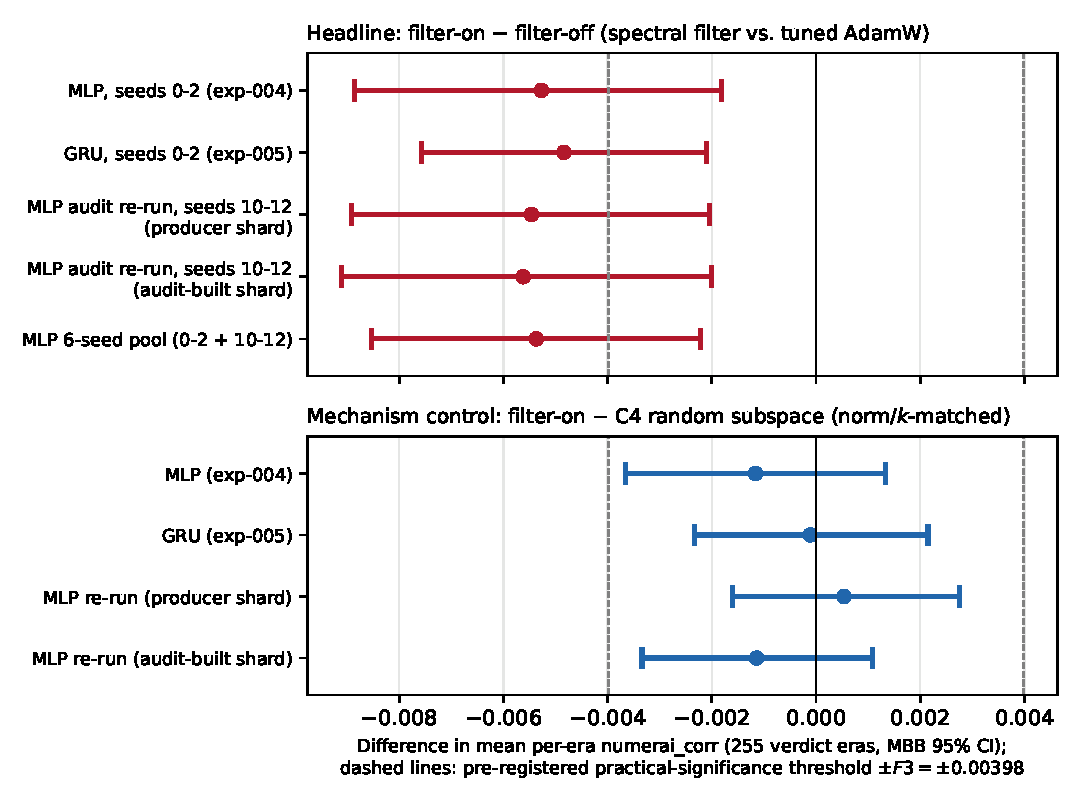
\includegraphics[width=0.95\linewidth]{figures/headline_forest.pdf}
  \caption{Forest plot of the run's principal paired comparisons (mean
    per-era \texttt{numerai\_corr} differences over 255 verdict eras,
    moving-block-bootstrap 95\% CIs). Top: the filter significantly
    degrades out-of-sample performance vs.\ tuned AdamW on both
    architectures, and the result reproduces under the audit's fresh-seed
    re-execution on two independently constructed evaluation shards.
    Bottom: the spectral filter is indistinguishable from its
    norm/$k$-matched random-subspace control everywhere.}
  \label{fig:forest}
\end{figure}

\subsection{Exp-001: gate bundle and the target-independence result}
\label{sec:exp001}

The first experiment bundled the infrastructure gates (integration smoke,
data/protocol construction, throughput) with the run's highest-$\lambda$
question: is spectral ``engagement'' on financial gradients meaningful? The
infrastructure gates all passed (filter-off reproduces plain AdamW to fp64
precision; 31\,ms/step filter-on at $B{=}1024$ on one L40; 643 usable
validation eras). The headline engagement gate is logged as a
\textbf{FAIL on its C2 conjunct}---a pre-registered pass criterion
requiring real-target and permuted-target engagement spectra to be
distinguishable---and this failure is the run's first mechanistic
contribution.

Mechanically, the filter is healthy and selective on real financial
gradients: for every threshold mode $\times$ batch size $\times$ batch
composition, $0 < k < B$ on 100\% of logged steps ($k$ settling at 3--7),
kept-energy fraction 0.29--0.89, and the C3 cosine diagnostics show the
filtered update is not mean-gradient smoothing (median cosine 0.25--0.83;
the $>0.95$ degeneracy pivot never fired). The pre-registered \emph{hard}
fail-fast trigger therefore did not fire. But the C2 permuted-target
control was indistinguishable from real targets---provably so:

\begin{theorem}[Target independence of the engagement spectrum]
\label{thm:target-independence}
Let $f_\theta$ be a scalar-output model trained with per-sample MSE, so the
per-sample gradient is $g_i = 2\,(f_\theta(x_i) - y_i)\,\nabla_\theta
f_\theta(x_i)$. After row normalization, $\hat g_i =
\operatorname{sign}(f_\theta(x_i) - y_i)\,\nabla f_i / \lVert \nabla f_i
\rVert$. Hence for any targets $y'$ at the same parameter point, the
similarity matrix satisfies $S(y') = D\,S(y)\,D$ with $D =
\operatorname{diag}(\pm 1)$ orthogonal. The eigenspectrum of $S$---and
therefore $k$, the MP-threshold count, the kept-energy fraction, and every
spectrum-derived engagement diagnostic---is exactly target-independent at
fixed parameters.
\end{theorem}

The proof was verified numerically in fp64 (max eigenvalue difference
$8.9 \times 10^{-16}$ under target permutation; $1.3\times10^{-15}$ under
entirely different targets) and independently re-verified by the results
audit with a different construction ($2.1\times10^{-14}$), together with two
scoping controls showing the theorem is non-vacuous and correctly scoped:
the \emph{unnormalized} spectrum is strongly target-dependent
(difference $\approx 61$), and a 2-output MSE head breaks the invariance
(difference $\approx 0.61$). Targets influence the spectrum only through
the parameter trajectory, which at this horizon/SNR does not measurably
diverge: late-training real-vs-permuted diagnostic distributions are
statistically indistinguishable (the two nominally significant tests out of
twelve point in opposite directions), and end-of-run training loss on real
targets is not below permuted-target loss.

Two scoping notes. First, the update \emph{direction} does depend on
targets (through residual signs and magnitudes); what fails is the ability
of the engagement diagnostics to certify that the mechanism found target
signal---the premise for interpreting any engagement-gated verdict. Second,
the theorem is specific to scalar-output per-sample losses with row
normalization; multi-class cross-entropy gradients (the prior project's
MNIST label-noise setting) are \emph{not} scalar multiples of a
target-independent vector, which cleanly explains why the same diagnostics
were informative there and are not here. A synthetic calibration test
(C1) exhibits the failure mode directly: in hard mode the filter correctly
discards i.i.d.\ noise and keeps a planted spike, but also keeps a
correlated \emph{zero-signal} confound at cosine 0.96 to the confound
direction---and Theorem~\ref{thm:target-independence} says the real data is
the confound case, fully. Two additional observations from this gate recur
later: the similarity spectrum undergoes strong target-independent rank
collapse during training (one direction accumulating $\sim$80--90\% of the
mass), and the filter frequently \emph{amplifies} the update
(norm ratio $>1$ on 25--70\% of steps)---it is not shrinkage.

Following the pre-registered fail semantics, the run proceeded to the
comparison under an amended interpretation frame recorded before any
unblinding: the proof is a co-primary deliverable; any verdict is
attributed to target-blind spectral-subspace regularization, never
``consensus on signal''; and the C4 random-subspace control is
load-bearing. Binding registrations made at this gate from diagnostics
only: threshold mode \emph{hard} (mp\_factor 2.0), within-era batch
composition.

\subsection{Exp-002: sequence-arm feasibility}
\label{sec:exp002}

A hand-rolled functional GRU cell was validated for per-sample gradients
under \texttt{vmap(grad)}: element-wise agreement with a per-sample loop
reference to $1.7\times10^{-6}$ (tolerance $10^{-5}$) at $B{=}64$; a full
filtered step took 1.17\,s on CPU at $B{=}1024$, projecting well under the
job cap on an L40. This authorized the architecture-consistency arm
(exp-005) rather than an MLP-only fallback. The correctness assert was
re-run on-cluster at job start (max difference $4.8\times10^{-7}$).

\subsection{Exp-003: baseline sanity, power, and the go/no-go gate}
\label{sec:exp003}

A 12-trial AdamW sweep on tuning-block eras only produced best configuration
\texttt{t07} with mean per-era \texttt{numerai\_corr} $+0.0196$
(3-seed mean $+0.01594$; winner's-curse shrinkage $\sim$19\%), inside the
recalibrated sanity band; the zero-predictor was $\approx 0$ and the leakage
gate did not fire. From these outputs the verdict threshold was frozen at
$F3 = 0.00398$, the block length at $L{=}4$ (measured lag-1 autocorrelation
$+0.25$), and a moving-block-bootstrap power simulation of the paired
3-seed design at 255 verdict eras gave a median CI half-width of 0.00219
with $P(\text{some verdict category reachable}) = 0.910 \geq 0.6$
(go/no-go gate: GO; detection probability $\approx 0.90$--$0.92$ at
$\pm F3$). Two under-exploration signatures were recorded here, before
unblinding, and bind the wording of any negative verdict: the baseline's
best weight-decay and dropout sit at the grid boundary with improving
trends (the baseline itself may be slightly under-tuned---fixing this would
strengthen the negative), and the compute-matched budget affords the
spectral arm only $\sim$1 tuning trial vs.\ AdamW's 12 (the asymmetry that
mandates the F12 downgrade).

\subsection{Exp-004: the verdict experiment (MLP)}
\label{sec:exp004}

The first and only unblinding of the 255 verdict eras, with all arms and
configurations frozen beforehand. Table~\ref{tab:arms} gives arm levels;
the paired headline is in Table~\ref{tab:headline}. All three per-seed
headline differences are negative (seed-2 CI touches zero:
$[-0.01069, +0.00023]$); direction is seed-consistent.

\begin{table}[t]
\centering
\footnotesize
\begin{tabular}{lcccc}
\toprule
Arm & \texttt{numerai\_corr} & Spearman & corr-Sharpe & per-seed nc \\
\midrule
filter-off (tuned AdamW) & $+0.00641$ & $+0.00698$ & $0.309$ & $+0.0053$ / $+0.0066$ / $+0.0073$ \\
filter-on (spectral) & $+0.00113$ & $+0.00090$ & $0.109$ & $+0.0006$ / $+0.0007$ / $+0.0021$ \\
C4 random-subspace & $+0.00229$ & $+0.00112$ & $0.178$ & $+0.0004$ / $+0.0022$ / $+0.0043$ \\
GAF-style sign-agreement & $-0.00042$ & $+0.00004$ & $-0.032$ & $-0.0015$ / $+0.0012$ / $-0.0009$ \\
zero-predictor & $+0.00063$ & $+0.00057$ & --- & sanity $\approx 0$ \\
\bottomrule
\end{tabular}
\caption{Exp-004 arm levels (mean per-era scores over 255 verdict eras,
  3-seed means, MLP).}
\label{tab:arms}
\end{table}

\textbf{Mechanism attribution (the load-bearing control).} The spectral
filter is statistically indistinguishable from its norm- and $k$-matched
random-subspace control ($-0.00116$, CI $[-0.00366, +0.00134]$)---an
equivalence claim at the $\pm 0.004$ resolution the design affords, not an
identity claim. All three filtered arms hurt by similar amounts
($-0.0041$ to $-0.0068$ vs.\ baseline) despite very different mechanisms
(eigenspectral, random-subspace, coordinate sign-agreement):
per-sample-agreement-style update modification \emph{as a class} degrades
out-of-sample performance in this regime. Combined with
Theorem~\ref{thm:target-independence}, the account is closed from both
ends: the selection is target-blind by proof, and its effect is no
different from projecting onto a random sample-subspace with the same
kept-$k$ and norm trajectory.

\textbf{Engagement during the verdict runs.} The filter did real, selective
work throughout (selective on 100\% of logged steps): $k$ collapsed from
$\sim$52 at step 0 to a median of $\sim$1, with update-norm ratio
$\sim$9.5--13.9$\times$ the mean gradient---the filter effectively replaced
the averaged gradient with a single amplified dominant eigendirection.
The C4 control matched exactly this $(k, \text{ratio})$ trajectory, which
is what makes the null comparison meaningful. The a-priori plausible
``implicit regularization by norm shrinkage'' story is inverted here: the
filter amplifies.

\textbf{Tail-era breakdowns.} Bucketing eras by the baseline's own realized
per-era corr shows a strong monotone gradient (filter ``helps'' on the
baseline's worst quartile, $+0.019$; hurts most on its best, $-0.030$), but
this split is outcome-conditioned and mechanically contaminated by
regression to the mean (flagged in the analysis code before results); we
report it as descriptive only. The evidentially meaningful, unconditioned
split by per-era \emph{target dispersion} shows roughly uniform harm across
quartiles---no evidence of the Feldman-style pattern
\citep{feldman2019longtailmemorization} in which harm concentrates in
high-dispersion (tail) eras. The corr-Sharpe also fell, so the filter did
not buy stability either.

\textbf{Sanity notes.} The realized verdict-block baseline ($+0.00641$)
sits \emph{below} the tuning-block sanity band $[0.0087, 0.0522]$; the
leakage gate did not fire. The verdict eras are a genuinely harder, later
regime (the example model also drops from 0.0418 to 0.0235 between
blocks)---this regime drift scopes the claim
(Section~\ref{sec:limitations}) and made the frozen threshold a $\sim$62\%
relative bar rather than the intended 25\%; the verdict does not depend on
it (the CI excludes zero regardless).

\subsection{Exp-005: architecture consistency (GRU)}
\label{sec:exp005}

The same data, shards, seeds, frozen thresholds, and inference machinery,
with the only change being the architecture (within-era Numerai framing,
$15 \times 47$ reshape; the supported claim is \emph{architecture
consistency}, not ``second setting''). The GRU reproduces the MLP's result:
headline $-0.00484$, CI $[-0.00758, -0.00211]$ (same category, F12
downgrade applied identically); spectral-vs-random null replicates even
more tightly ($-0.00011$, CI $[-0.00233, +0.00215]$); corr-Sharpe
$-0.242$, CI $[-0.414, -0.073]$ (robust); the dispersion split again shows
no tail pattern. All six per-seed headline differences across both
experiments are negative.

Notably, the filter engages in a \emph{different regime} on the GRU
($k \approx 60$ kept directions, mild attenuation at norm ratio
0.80--0.85) than on the MLP ($k \approx 1$, $\sim$10$\times$
amplification), yet produces near-identical harm and the same null against
the random-subspace control---strengthening the account that the harm
tracks the generic subspace-projection/rescaling intervention class rather
than any particular spectral selection or amplification behavior. The GRU
arms ran at the \texttt{t07} configuration transferred from the MLP
(frozen pre-unblinding and identical across arms, so the paired comparison
is protocol-valid; the skipped GRU sweep is a recorded limitation,
Section~\ref{sec:limitations}). The untuned GRU baseline ($+0.00586$)
landed within $\sim$9\% of the tuned MLP baseline despite 9$\times$ fewer
parameters.

\subsection{Robustness: independent audit re-execution}
\label{sec:robustness}

An independent results audit re-executed the load-bearing exp-004 on the
cluster using the producer's frozen code with \textbf{fresh seeds
\{10, 11, 12\}} and, additionally, an \textbf{auditor-built verdict shard}
subsampled independently from the raw validation parquet (different RNG;
the producer's shard was also row-matched against the raw parquet, ruling
out fabrication). The headline reproduces in category, direction, and
magnitude on both shards ($-0.00546$ and $-0.00562$ vs.\ the original
$-0.00527$), the 6-seed pooled headline is $-0.00537$, CI
$[-0.00853, -0.00222]$, and the C4 spectral-vs-random null replicates
(Table~\ref{tab:headline}; all audit CIs from independent bootstrap code).
The audit also independently re-verified Theorem~\ref{thm:target-independence}
and re-derived every reported number from primary artifacts (robustness
cross-checks: paired $t$-test $p = 1.5\times10^{-4}$, Wilcoxon
$p = 1.8\times10^{-4}$).

The re-execution surfaced one implementation defect that the original runs
did not hit: under the rank-collapse regime this study itself documents
(one eigenvalue carrying $\sim$80--90\% of the mass), fp32
\texttt{linalg.eigh} on GPU can fail to converge, crashing the run
stochastically by seed. The original 6-of-6 producer runs completed without
encountering it; the audit's mathematically equivalent CPU-fp64 fallback
(which fired on 4 of 18{,}000 filtered steps) completed the re-run and
reproduced all conclusions. This is an availability defect of the released
implementation, not a bias in the reported numbers; it is disclosed in
Section~\ref{sec:limitations}.
